% Options for packages loaded elsewhere
\PassOptionsToPackage{unicode}{hyperref}
\PassOptionsToPackage{hyphens}{url}
%
\documentclass[
]{book}
\usepackage{amsmath,amssymb}
\usepackage{lmodern}
\usepackage{iftex}
\ifPDFTeX
  \usepackage[T1]{fontenc}
  \usepackage[utf8]{inputenc}
  \usepackage{textcomp} % provide euro and other symbols
\else % if luatex or xetex
  \usepackage{unicode-math}
  \defaultfontfeatures{Scale=MatchLowercase}
  \defaultfontfeatures[\rmfamily]{Ligatures=TeX,Scale=1}
\fi
% Use upquote if available, for straight quotes in verbatim environments
\IfFileExists{upquote.sty}{\usepackage{upquote}}{}
\IfFileExists{microtype.sty}{% use microtype if available
  \usepackage[]{microtype}
  \UseMicrotypeSet[protrusion]{basicmath} % disable protrusion for tt fonts
}{}
\makeatletter
\@ifundefined{KOMAClassName}{% if non-KOMA class
  \IfFileExists{parskip.sty}{%
    \usepackage{parskip}
  }{% else
    \setlength{\parindent}{0pt}
    \setlength{\parskip}{6pt plus 2pt minus 1pt}}
}{% if KOMA class
  \KOMAoptions{parskip=half}}
\makeatother
\usepackage{xcolor}
\IfFileExists{xurl.sty}{\usepackage{xurl}}{} % add URL line breaks if available
\IfFileExists{bookmark.sty}{\usepackage{bookmark}}{\usepackage{hyperref}}
\hypersetup{
  pdftitle={Digital Skills Primer},
  pdfauthor={Aaron McMurray},
  hidelinks,
  pdfcreator={LaTeX via pandoc}}
\urlstyle{same} % disable monospaced font for URLs
\usepackage{longtable,booktabs,array}
\usepackage{calc} % for calculating minipage widths
% Correct order of tables after \paragraph or \subparagraph
\usepackage{etoolbox}
\makeatletter
\patchcmd\longtable{\par}{\if@noskipsec\mbox{}\fi\par}{}{}
\makeatother
% Allow footnotes in longtable head/foot
\IfFileExists{footnotehyper.sty}{\usepackage{footnotehyper}}{\usepackage{footnote}}
\makesavenoteenv{longtable}
\usepackage{graphicx}
\makeatletter
\def\maxwidth{\ifdim\Gin@nat@width>\linewidth\linewidth\else\Gin@nat@width\fi}
\def\maxheight{\ifdim\Gin@nat@height>\textheight\textheight\else\Gin@nat@height\fi}
\makeatother
% Scale images if necessary, so that they will not overflow the page
% margins by default, and it is still possible to overwrite the defaults
% using explicit options in \includegraphics[width, height, ...]{}
\setkeys{Gin}{width=\maxwidth,height=\maxheight,keepaspectratio}
% Set default figure placement to htbp
\makeatletter
\def\fps@figure{htbp}
\makeatother
\setlength{\emergencystretch}{3em} % prevent overfull lines
\providecommand{\tightlist}{%
  \setlength{\itemsep}{0pt}\setlength{\parskip}{0pt}}
\setcounter{secnumdepth}{5}
\usepackage{booktabs}
\ifLuaTeX
  \usepackage{selnolig}  % disable illegal ligatures
\fi
\usepackage[]{natbib}
\bibliographystyle{apalike}

\title{Digital Skills Primer}
\author{Aaron McMurray}
\date{2022-06-10}

\begin{document}
\maketitle

{
\setcounter{tocdepth}{1}
\tableofcontents
}
\hypertarget{A-Note-About-this-Resource}{%
\chapter*{A Note About this Resource}\label{A-Note-About-this-Resource}}
\addcontentsline{toc}{chapter}{A Note About this Resource}

\begin{center}\rule{0.5\linewidth}{0.5pt}\end{center}

\textbf{What is this?}

This resource has been produced using a combination of \textbf{R}, \textbf{LaTeX} and \textbf{R Studio} and published through \textbf{GitHub} by converting the content to \textbf{HTML}. Publishing this way supports the embedding of images, video content, html content (iframes), live code and mathematical formula and makes sharing the content much easier.

Currently, this resource details statistics to serve as an example of the type of dynamic content that can be created by hosting and publishing through GitHub, however this resource could be developed into a \textbf{Digital Skills Primer} resource covering \textbf{Microsoft Power BI, Python, R, Flourish, Genially}. This Primer would serve as a singular point of reference for digital tools currently being used for research and data visualisation. This could be useful for current staff working with these tools and new staff, temporary staff and students who may not have received training on these tools. There is a wealth of documentation being developed for accessibility and style but no singular point of reference for the tools which are to be made accessible and stylised!

The aim would not be to produce a prescriptive document detailing how users must use these products but instead provide a resource with information, tutorials, summaries and answers to frequently asked questions that would take users from zero knowledge to proficiency with the digital tools being used in research. Now is also an ideal time to develop something like this and from various conversations there is significant interest in something like this being developed.

\textbf{Why host on GitHub?}

As the resource is hosted on GitHub it is available anywhere, any time and on any device facilitating mobile working. In addition, users with a GitHub account can `fork' the repository to look at the code used to generate this resource and build and improve on it in their own way facilitating greater collaboration and transparency. Alternatively they can suggest changes to the code, which can then be reviewed and approved, facilitating greater collaboration on projects like this.

GitHub does not need to be used to produce documentation, it can also host stand alone scripts written in any programming language which other users can fork or suggest changes to. The UK Government has several GitHub accounts, the most prominent being the \href{https://github.com/alphagov}{Government Digital Service GitHub} which is used to store and collaborate on code used to build platforms, products and services that help deliver ``a simple, joined-up and personalised experience of government to everyone''.

The Repository hosting this resource can be found at \href{https://github.com/aamcmurray/BookTest}{github.com/aamcmurray/BookTest}. Other users with a GitHub account can suggest changes which can be approved or denied by the repository owner.

A repository for our department could be used to store code developed by staff (for instance, scripts I developed to make API calls, automate data cleaning and calculation of moving averages and perform web scraping). This means that the code would be accessible to everyone to use and adapt for their own purposes.

GitHub hosting also means anybody can contribute to this making this document one that can evolve and change over time and one that is owned by everybody.

\textbf{\emph{Sounds Complicated\ldots{}}}

To develop this further all that is needed is to sign an e-mail up for a free GitHub account. There is no need for complicated software installations or purchasing new software.

\hypertarget{Introduction-to-Statistics}{%
\chapter*{Introduction to Statistics}\label{Introduction-to-Statistics}}
\addcontentsline{toc}{chapter}{Introduction to Statistics}

\begin{center}\rule{0.5\linewidth}{0.5pt}\end{center}

\textbf{Overview}

This resource is intended to provide an introduction to the basics of statistics.

\textbf{Contents}

\begin{itemize}
\tightlist
\item
  Introduction
\item
  Data Types and Levels of Measurement
\item
  Describing Data
\item
  Comparing Data
\item
  Data Visualisation
\item
  Correlation
\item
  Sampling
\item
  Confidence Intervals
\item
  Hypothesis Testing
\item
  Statistical Significance
\item
  Odds against Chance Fallacy
\item
  Statistical Significance Verses Importance
\end{itemize}

\hypertarget{intro}{%
\chapter{Introduction}\label{intro}}

\begin{center}\rule{0.5\linewidth}{0.5pt}\end{center}

\hypertarget{what-is-statistics}{%
\section{What is Statistics?}\label{what-is-statistics}}

Statistics is all about the collection, organization, analysis, interpretation and presentation of data. Statistics is used everywhere from opinion polling in politics to predicting the prices of assets. There are two main branches of statistics: descriptive statistics and inferential statistics.

\hypertarget{descriptive-statistics}{%
\section{Descriptive Statistics}\label{descriptive-statistics}}

Descriptive statistics describes or summarises data that have been collected. Measures of central tendency such as (mean, median and the mode) and measures of dispersion (range, interquartile range and standard deviation) are the most important tools.

\hypertarget{inferential-statistics}{%
\section{Inferential Statistics}\label{inferential-statistics}}

Inferential statistical is used to make prediction about a population using information gathered about a sample. Inferential statistics involves hypothesis testing and regression analysis.

\hypertarget{data-types-and-levels-of-measurement}{%
\chapter{Data Types and Levels of Measurement}\label{data-types-and-levels-of-measurement}}

\begin{center}\rule{0.5\linewidth}{0.5pt}\end{center}

\hypertarget{types-of-data}{%
\section{Types of Data}\label{types-of-data}}

Data can be broadly categorised as \textbf{qualitative} (data relating to qualities or characteristics) or quantitative (numerical data relating to sizes or quantities of things).

We can further categorise \textbf{quantitative} data as being continuous or discrete.

\textbf{Discrete} data involves whole numbers that can't be divided because of what they represent (number of people in a class, number of cars owned). The number of people in a class cannot be 10.5 or 3.14. It must be a whole number because people are not divisible.

\textbf{Continuous} data can be divided and measured to some number of decimal places (height, weight, speed in miles per hour). A person's height can be any number (provided it lies within the range of possible human heights) and can be reported to any number of decimal places (150cm or 150.1cm or 150.12cm) depending on how accurate the measurement tool is.

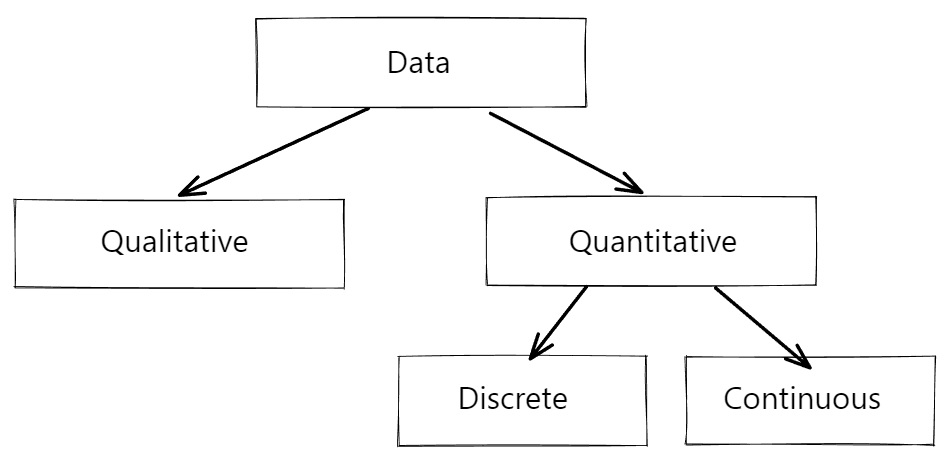
\includegraphics{data.jpg}
There are also different \textbf{levels of measurement}.

\hypertarget{levels-of-measurement}{%
\section{Levels of Measurement}\label{levels-of-measurement}}

The levels of measurement describe how precisely variables are recorded. The different levels of measurement limit which statistics can be used to summarise data and which inferential statistics can be performed. These levels are:

\begin{itemize}
\tightlist
\item
  Nominal
\item
  Ordinal
\item
  Interval
\item
  Ratio
\end{itemize}

\hypertarget{nominal}{%
\subsection{Nominal}\label{nominal}}

\textbf{Nominal data} is a type of data that is used to label variables. It can be categorised but not ranked (eye colour and gender for instance). The values grouped into these categories have no meaningful order. It is not possible to form a meaningful hierarchy of gender or eye colour.

\begin{figure}

{\centering 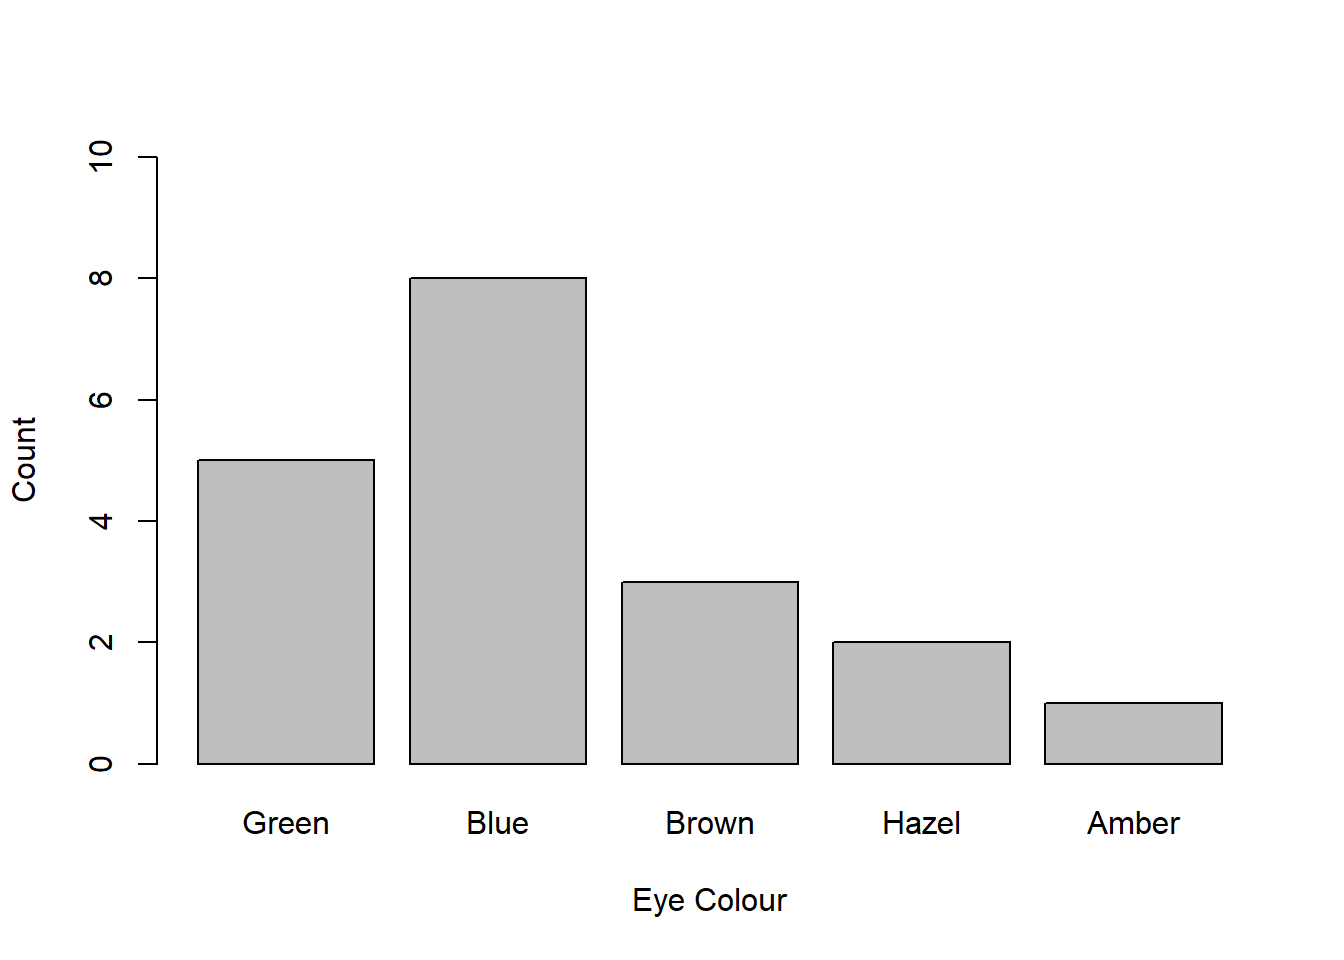
\includegraphics{Bookdown_files/figure-latex/chunk-label-1} 

}

\caption{Eye colour is an example of nominal data.}\label{fig:chunk-label}
\end{figure}

The only measure of central tendency used with nominal data is the mode.

\hypertarget{ordinal}{%
\subsection{Ordinal}\label{ordinal}}

\textbf{Ordinal data} is another type of \textbf{qualitative data} that groups variables into descriptive categories. The categories used for ordinal data are ordered in some kind of hierarchical scale although the distance between those categories may be uneven or even unknown.

\begin{figure}

{\centering 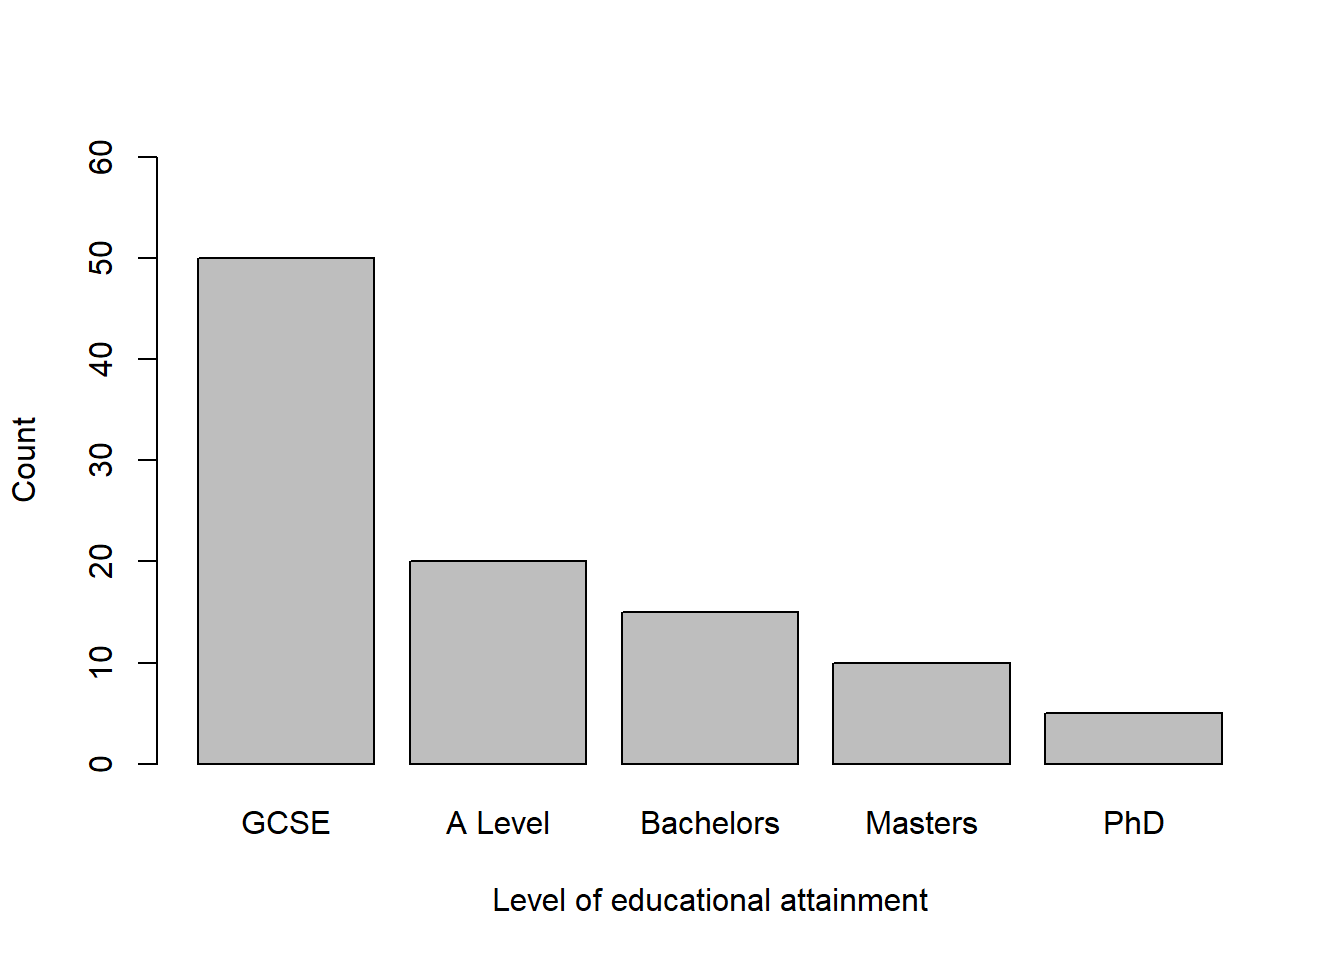
\includegraphics{Bookdown_files/figure-latex/unnamed-chunk-1-1} 

}

\caption{The highest level of educational attainment has a heirarchical scale but the distance between categories is unclear.}\label{fig:unnamed-chunk-1}
\end{figure}

Ordinal variables often include ratings about opinions that can be categorised (strongly agree, agree, don't know, disagree, strongly disagree).

The descriptive statistics which can be used with ordinal data are the mode and the median.

Ordinal data can also be described with a measure of dispersion, namely, range.

\hypertarget{interval}{%
\subsection{Interval}\label{interval}}

\textbf{Interval data} is a type of quantitative data that groups variables into categories. Values can be ordered and separated using an equal measure of distance.

An example of interval level data is temperature data recorded in Celsius or Fahrenheit. The values on either scale are ordered and separated using an equal measure of distance (the distances between notches on a thermometer are always equally spaced).

\begin{figure}

{\centering 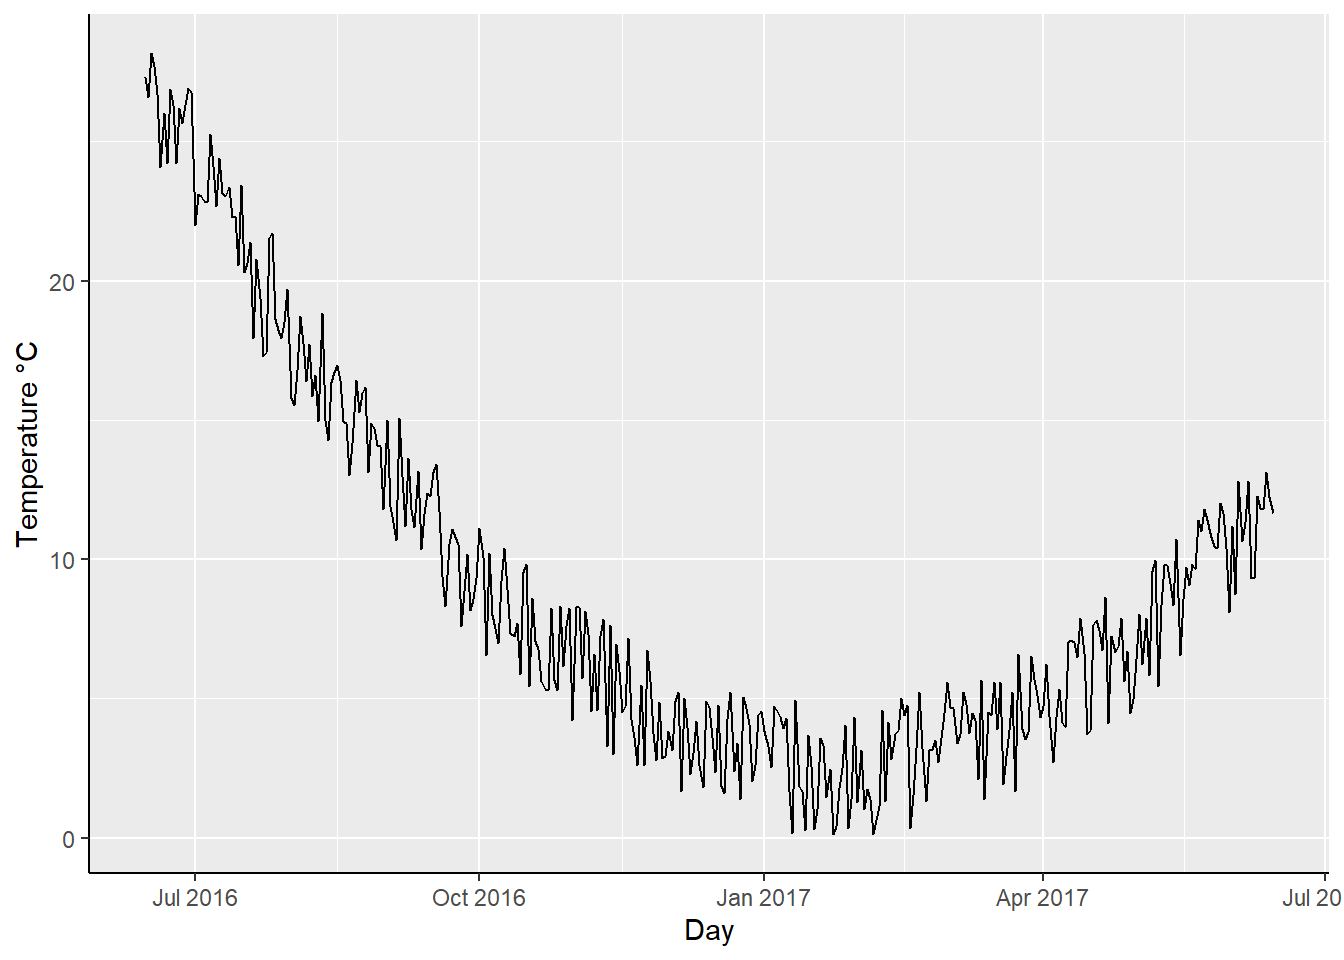
\includegraphics{Bookdown_files/figure-latex/unnamed-chunk-2-1} 

}

\caption{Temperature in Celsius is interval data. The values are ordered and separated by an equal interval. The distance between 0°C and 1°C is the same as the distance between 2°C and 3°C.}\label{fig:unnamed-chunk-2}
\end{figure}

Mathematical operations can be carried out on this type of data, for instance, subtracting one value from another to find the difference. Interval data lacks a \textbf{true zero}.

True zero indicates a lack of whatever is being measured. The Celsius scale doesn't qualify as having a true zero since the zero point in a thermometer is arbitrary. When the Celsius scale was first created by Anders Celsius 0°C was selected to match the boiling point of water and a value of 100 °C was the freezing point of water. The scale was later reversed. Thermometers measure heat and at 0°C there is still heat, maybe not a great deal of it but heat is still measurable meaning 0°C is not a true zero. The thermodynamic Kelvin Scale has a true zero - where particles have no motion and can become no colder (there is a true absence of heat).

A range of descriptive statistics can be used to describe interval data. The measures of central tendency applicable to interval data are the \textbf{mode, median} and the \textbf{mean}. The measures of dispersion applicable to interval data are the \textbf{range, standard deviation} and the \textbf{variance}.

\hypertarget{ratio}{%
\subsection{Ratio}\label{ratio}}

\textbf{Ratio data} is a form of quantitative data. It measures variables on a continuous scale with an equal distance between adjacent values (weight, height). Ratio data has a true zero. Ratio data is the most complex of the four data types.

\begin{figure}

{\centering 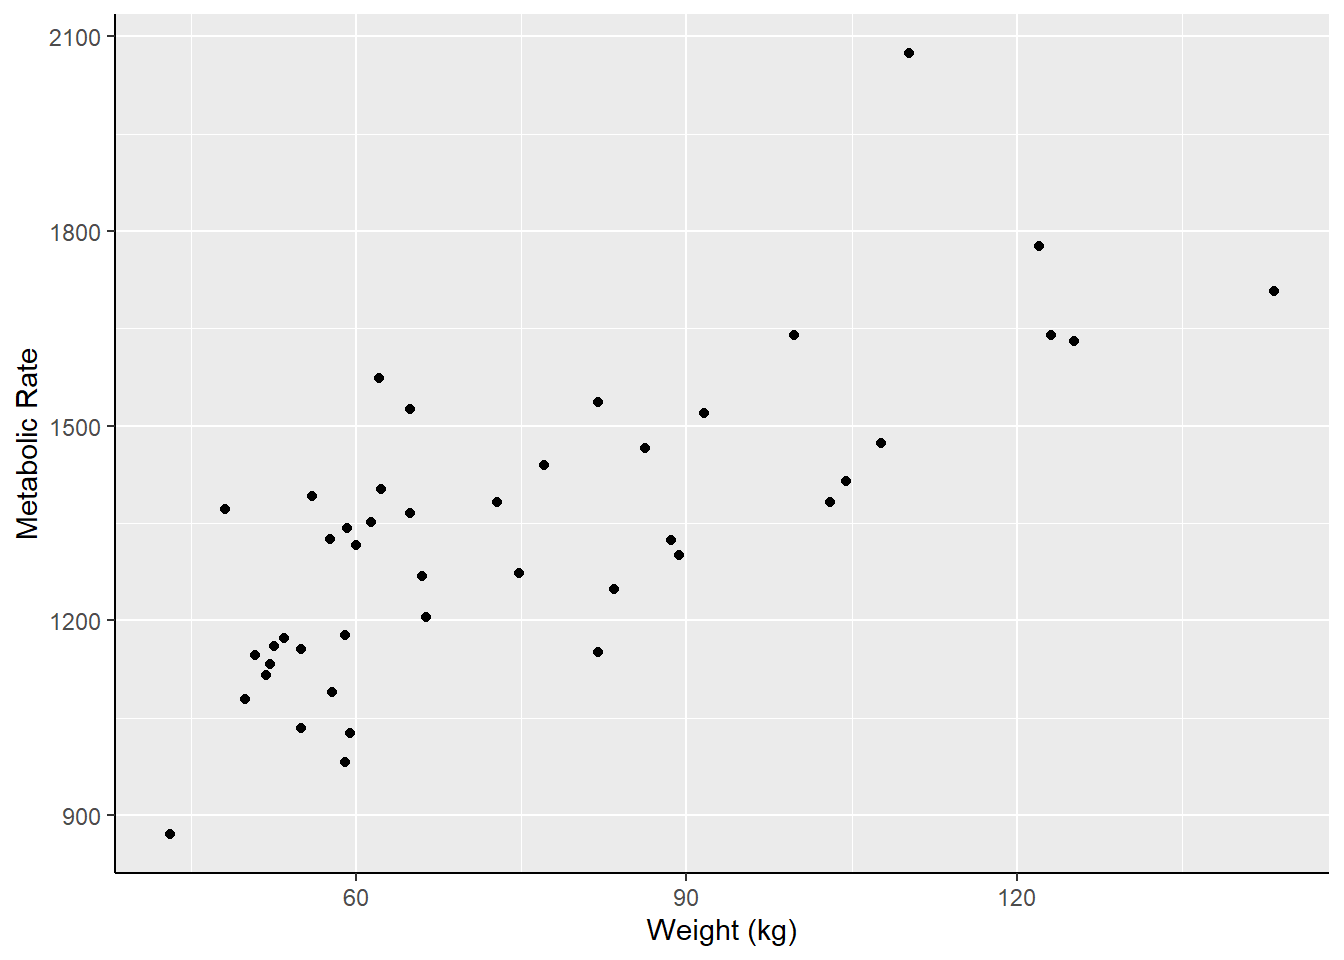
\includegraphics{Bookdown_files/figure-latex/unnamed-chunk-3-1} 

}

\caption{The scatterplot above shows metabolic rate plotted against body weight (kg). These are examples of ratio data. This data comes from the Introduction to Statistics with R (ISwR) library for R.}\label{fig:unnamed-chunk-3}
\end{figure}

Ratio data can be analysed with descriptive statistics including the \textbf{mode, median} and \textbf{mean}. \textbf{Range, standard deviation, variance} and the \textbf{coefficient of variation} can all be used to describe the dispersion of ratio data.

\hypertarget{describing-data}{%
\chapter{Describing Data}\label{describing-data}}

\begin{center}\rule{0.5\linewidth}{0.5pt}\end{center}

\hypertarget{frequency}{%
\section{Frequency}\label{frequency}}

The \textbf{frequency} of an observation is the number of times it occurs or is recorded.A frequency table, like the one shown below detailing exam grades, is a commonly used method of depicting frequency.

\begin{longtable}[]{@{}rr@{}}
\caption{\label{tab:table2}Frequency Table}\tabularnewline
\toprule
Grade & Frequency \\
\midrule
\endfirsthead
\toprule
Grade & Frequency \\
\midrule
\endhead
A & 15 \\
B & 20 \\
C & 25 \\
D & 21 \\
E & 14 \\
\bottomrule
\end{longtable}

The total of all frequencies so far in a frequency distribution is the \textbf{cumulative frequency}. It is the `running total' of frequencies.

\begin{longtable}[]{@{}rrr@{}}
\caption{\label{tab:table3}Cumulative Frequency Table}\tabularnewline
\toprule
Grade & Frequency & Cumulative Frequency \\
\midrule
\endfirsthead
\toprule
Grade & Frequency & Cumulative Frequency \\
\midrule
\endhead
A & 15 & 15 \\
B & 20 & 35 \\
C & 25 & 60 \\
D & 21 & 81 \\
E & 14 & 95 \\
\bottomrule
\end{longtable}

The \textbf{relative frequency} is the ratio of the category frequency to the total number of outcomes. For grade A, the relative frequency is:

\[ \frac{15}{15+20+25+21+14}=0.16. \]

The table can be extended to include the relative frequency.

\begin{longtable}[]{@{}rrr@{}}
\caption{\label{tab:table4}Relative Frequency Table}\tabularnewline
\toprule
Grade & Frequency & Relative Frequency \\
\midrule
\endfirsthead
\toprule
Grade & Frequency & Relative Frequency \\
\midrule
\endhead
A & 15 & 0.16 \\
B & 20 & 0.21 \\
C & 25 & 0.26 \\
D & 21 & 0.22 \\
E & 14 & 0.15 \\
\bottomrule
\end{longtable}

The \textbf{relative frequency} can be reported as a percentage by multiplying the values by 100\%. For grade A, the relative frequency reported as a percentage is: 100\% x 0.16 = 16\%.

\hypertarget{measures-of-central-tendency}{%
\section{Measures of Central Tendency}\label{measures-of-central-tendency}}

Measures of central tendency help find the middle, or the average, of a data set.The measures of central tendency are the mean, median and mode.

\hypertarget{mean}{%
\subsection{Mean}\label{mean}}

The mean is the sum of the recorded values divided by the number of values recorded.

\hypertarget{example}{%
\subsubsection{Example}\label{example}}

Find the mean of this list of numbers:

\[ 2, 3, 3, 4, 20.\]
\[ \textrm{Mean} = \frac{\textrm{Sum of recorded values}}{\textrm{Number of values recorded}},\]
\[ \textrm{Mean} = \frac{\textrm{2 + 3 + 3 + 4 + 20}}{\textrm{5}},\]
\[ \textrm{Mean} = \frac{\textrm{32}}{\textrm{5}},\]

\[ \textrm{Mean} = 6.4.\]

\hypertarget{median}{%
\subsection{Median}\label{median}}

The \textbf{median} is the middle number in a sorted, ascending or descending, list of values.

If there are an odd number of values the median is simply the middle value.

For an even number of values there will be two values in the center. Those values are summed and divided by two.

The median is sometimes used as opposed to the mean when there are outliers that might skew the average of the values.

\hypertarget{example-1}{%
\subsubsection{Example}\label{example-1}}

Find the median of this list of numbers:

\[ 2, 3, 3, 4, 20.\]

There are 5 values listed in ascending order and the middle value is the third value in the list so the median is 3.

Note: In the previous example the mean was 6.4. It was skewed by the outlier (20). The median remains closer to what might be considered to be the middle of the data set.

\hypertarget{example-2}{%
\subsubsection{Example}\label{example-2}}

Find the median of this list of numbers:

\[ 3, 5, 4, 4, 2, 8, 7, 1.\]

The list should be sorted:

\[ 1, 2, 3, 4, 4, 5, 7, 8. \]

There are an even number of values so there will be two middle values. The middle values are 4 and 4. Sum them and divide by two to get the median: 4.

\hypertarget{mode}{%
\subsection{Mode}\label{mode}}

The mode of a set of data values is the value that appears most often. It is the value that is most likely to be sampled. There can be multiple modes or no modes.

\hypertarget{example-3}{%
\subsubsection{Example}\label{example-3}}

Find the mode of this list of numbers:

\[ 1, 2, 2, 2, 3, 3, 4.\]

A simple way to find the mode is to make a frequency table with the unique values on the left hand side and their frequency on the right hand side. We can tally up how many times each number occurs. Whichever has the greatest frequency is our mode.

\begin{longtable}[]{@{}rr@{}}
\caption{\label{tab:table5}}\tabularnewline
\toprule
Value & Frequency \\
\midrule
\endfirsthead
\toprule
Value & Frequency \\
\midrule
\endhead
1 & 1 \\
2 & 3 \\
3 & 2 \\
4 & 1 \\
\bottomrule
\end{longtable}

The mode is 2.

\hypertarget{example-4}{%
\subsubsection{Example}\label{example-4}}

Find the mode of this list of numbers:

\[ 7, 3, 5, 3, 4, 3, 5, 6, 8, 5.\]

\begin{longtable}[]{@{}rr@{}}
\caption{\label{tab:table6}}\tabularnewline
\toprule
Value & Frequency \\
\midrule
\endfirsthead
\toprule
Value & Frequency \\
\midrule
\endhead
3 & 3 \\
4 & 1 \\
5 & 3 \\
6 & 1 \\
7 & 1 \\
8 & 1 \\
\bottomrule
\end{longtable}

This is \textbf{bimodal}, it has two modes, 3 and 5.

\hypertarget{example-5}{%
\subsubsection{Example}\label{example-5}}

Find the mode of this list of numbers:

\[ 1, 2, 3, 4, 5, 6.\]

\begin{longtable}[]{@{}rr@{}}
\caption{\label{tab:table7}}\tabularnewline
\toprule
Value & Frequency \\
\midrule
\endfirsthead
\toprule
Value & Frequency \\
\midrule
\endhead
1 & 1 \\
2 & 1 \\
3 & 1 \\
4 & 1 \\
5 & 1 \\
6 & 1 \\
\bottomrule
\end{longtable}

Every value is unique and occurs only once so this data has no mode.

\hypertarget{using-excel}{%
\subsection{Using Excel}\label{using-excel}}

It is useful to calculate descriptive statistics by hand for understanding but for larger data sets it is not always possible to arrange data and perform calculations by hand.

Excel has a number of functions designed to perform descriptive statistics.

\textbf{Frequency}

=FREQUENCY(start:end,bins\_array)

The frequency() function will return a frequency table describing your data. It takes two arguments, the first being the array of values and the second being an array describing the upper boundary of the bins used.

\textbf{Average}

=AVERAGE(start:end)

The mean is calculated using the average() function. There are several other functions relating to means: geomean(), harmean() and trimmean(). Take care not to use these as they are quite different from calculating the mean that has been described here.

\textbf{Median}

=MEDIAN(start:end)

The median is calculated using the median() function.

\textbf{Mode}

=MODE.SNGL(start:end)

=MODE.MULT(start:end)

There are several functions for calculating the mode: mode(), mode.sngl() and mode.mult().
mode() was used in Excel 2007 and may still appear as an option in some versions of Excel.
mode.sngl() will return one mode and mode.mult() will return multiple modes (if there are multiple modes).

Neither mode() nor mode.sngl() will warn you if there are multiple modes so mode.mult() is usually the safest option.

\hypertarget{example-6}{%
\subsubsection{Example}\label{example-6}}

In the example below, the variable name is in cell A1 and the values are in cells A2 to A18. To calculate the average, type ``=AVERAGE(A2:A18)'' in another cell. It doesn't matter which cell but in this example A19 has been used. Press enter to return the value.

\begin{figure}
\centering
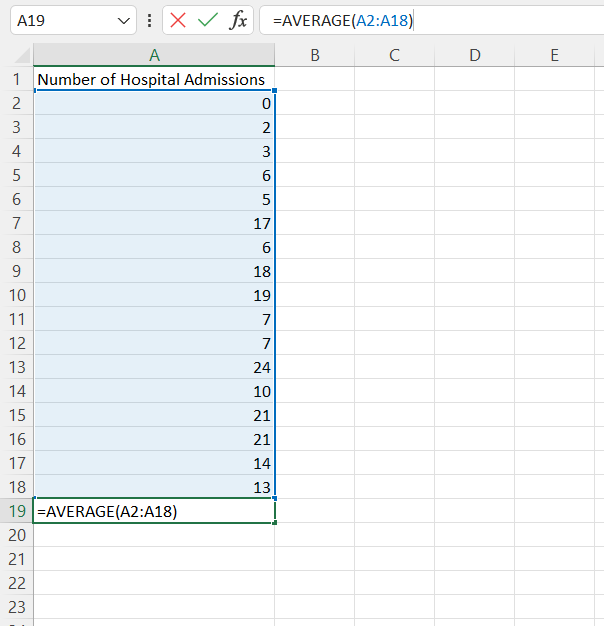
\includegraphics{Excelimage.png}
\caption{Screen shot showing excel spreadsheet with a list of values and the average being calculated using the average() function.}
\end{figure}

\hypertarget{measures-of-dispersion}{%
\section{Measures of Dispersion}\label{measures-of-dispersion}}

\textbf{Dispersion} (or variability) describes how far apart data points lie from each other and the center of a distribution. The \textbf{range, interquartile range, variance} and \textbf{standard deviation} are all measures of dispersion and they describe how far apart data points lie from one another and the center of a distribution.

\hypertarget{range}{%
\subsection{Range}\label{range}}

The range is the difference between the highest and lowest values and is calculated by subtracting the minimum value from the maximum value.

\hypertarget{example-7}{%
\subsubsection{Example}\label{example-7}}

Calculate the range for the following set of numbers:

\[ 23, 42, 75, 19, 74. \]
First, arrange the values in ascending order:

\[ 19, 23, 42, 74, 75. \]
The maximum value is 75 and the minimum is 19.

\[ \textrm{Range}= 75 - 19, \]
\[ \textrm{Range} = 56.\]

\hypertarget{interquartile-range}{%
\subsection{Interquartile Range}\label{interquartile-range}}

The \textbf{interquartile range} (IQR) describes the spread of the middle half of a distribution. How the interquartile range is calculated depends on whether there are an even or an odd number of values in a dataset.

For an even number of values the dataset in split half. The medians for the two new subsets of data are calculated. The positive difference of those medians is the interquartile range.
For an odd number of values either the inclusive or the exclusive method of finding the interquartile range must be used.

\begin{figure}
\centering
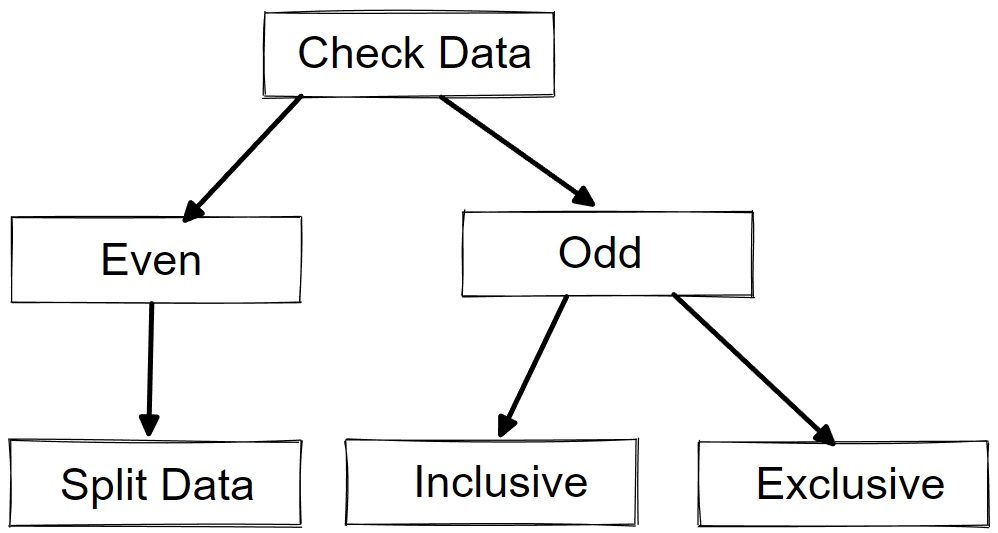
\includegraphics{iqrtree.jpg}
\caption{Tree diagram showing process of deciding how to calculate the IQR}
\end{figure}

The algorithm for the \textbf{exclusive method} is detailed below:

\begin{enumerate}
\def\labelenumi{\arabic{enumi}.}
\tightlist
\item
  Arrange the data in numeric order.
\item
  Remove the median and split the data about its center.
\item
  Find the medians of the two newly appended subsets of data.
\item
  Calculate the difference.
\end{enumerate}

The algorithm for the \textbf{inclusive method} is detailed below:

\begin{enumerate}
\def\labelenumi{\arabic{enumi}.}
\tightlist
\item
  Arrange the data in numeric order.
\item
  Remove the median and split the data about its center.
\item
  Append the two new subsets of data with the median.
\item
  Find the medians of the two newly appended subsets of data.
\item
  Calculate the difference.
\end{enumerate}

\hypertarget{example-8}{%
\subsubsection{Example}\label{example-8}}

\textbf{Even}

Find the interquartile range for the list of numbers below:

\[6, 7, 8, 8, 7, 6, 9, 5, 10, 4. \]
There are an even number of values. Arrange them in numeric order:

\[ 4, 5, 6, 6, 7, 7, 8, 8, 9, 10.\]
Split the values about their center into two sub sets of data.

\[ (4, 5, 6, 6, 7), (7, 8, 8, 9, 10). \]
Find the medians of each of these sub sets. The first subset has a median of 6 while the second has a median of 8.

The interquartile range is:

\[ \textrm{IQR} = 8 - 6 = 2.\]
Note: To calculate the interquartile range the smaller median value is always subtracted from the larger.

\textbf{Odd (Exclusive Method)}

Find the interquartile range for the list of numbers below:

\[2, 3, 2, 4, 3, 5, 4, 4, 2.\]
Arrange the values in numeric order:

\[2, 2, 2, 3, 3, 4, 4, 4, 5. \]
Remove the median (3) and split the data as before:

\[ (2, 2, 2, 3), (4, 4, 4, 5).\]
The interquartile range is:

\[ \textrm{IQR}=\textrm{Median of sub set 2}- \textrm{Median of sub set 1},\]
\[ \textrm{IQR}=\frac{4+4}{2} - \frac{2+2}{2}=\frac{8}{2} - \frac{4}{2} = 4 - 2= 2.\]
\textbf{Odd (Inclusive Method)}

Find the interquartile range of the list of numbers below:

\[ 2, 3, 2, 4, 3, 5, 4, 4, 2.\]
Sort in numeric order as before:

\[2, 2, 2, 3, 3, 4, 4, 4, 5.\]

Split the data as before but append each subset of data with the median (at the end and start of each subset respectively):

\[(2, 2, 2, 3, 3),(3, 4, 4, 4, 5).\]
Find the medians of each of the subsets and calculate the interquartile range. The median of the first subset is 2 and the median of the second subset is 4.

\[ \textrm{IQR} = 4 - 2 = 2 \]

The interquartile range is a useful measure of variability for skewed distributions. It can show where most values lie and how clustered they are. It is useful for datasets with outliers as it is based on the middle half of the distribution and less influenced by extreme values. Exclusive calculations result in a wider interquartile range than inclusive calculations.

\hypertarget{variance-and-standard-deviation}{%
\subsection{Variance and Standard Deviation}\label{variance-and-standard-deviation}}

The standard deviation describes to what extent a set of numbers lie apart (their spread). It is the square root of variance which is also an indicator of the spread of values.

\textbf{Variance}

To calculate the variance:
1. Start by finding the mean of the values in the dataset.
2. Find the difference between each recorded value and the mean.
3. Square those differences.
4. Sum the squared differences.
5. Divide the sum by the number of values recorded for population variance or the sum of the number of values minus 1 for sample variance.

\textbf{Standard Deviation}

Taking square root of the variance corrects for the fact that all the differences were squared, resulting in the standard deviation.

The plot below shows three distributions of values, each with a mean of 30 but with different standard deviations. In statistics there is a rule called the empirical rule that states that 68\%, 95\%, and 99.7\% of the values lie within one, two, and three standard deviations of the mean, respectively.

To make sense of this through an example, the plot below shows some simulated data for test scores. Three groups given the same test could achieve the same average score but with greater or lesser spreads of scores.

\begin{figure}

{\centering 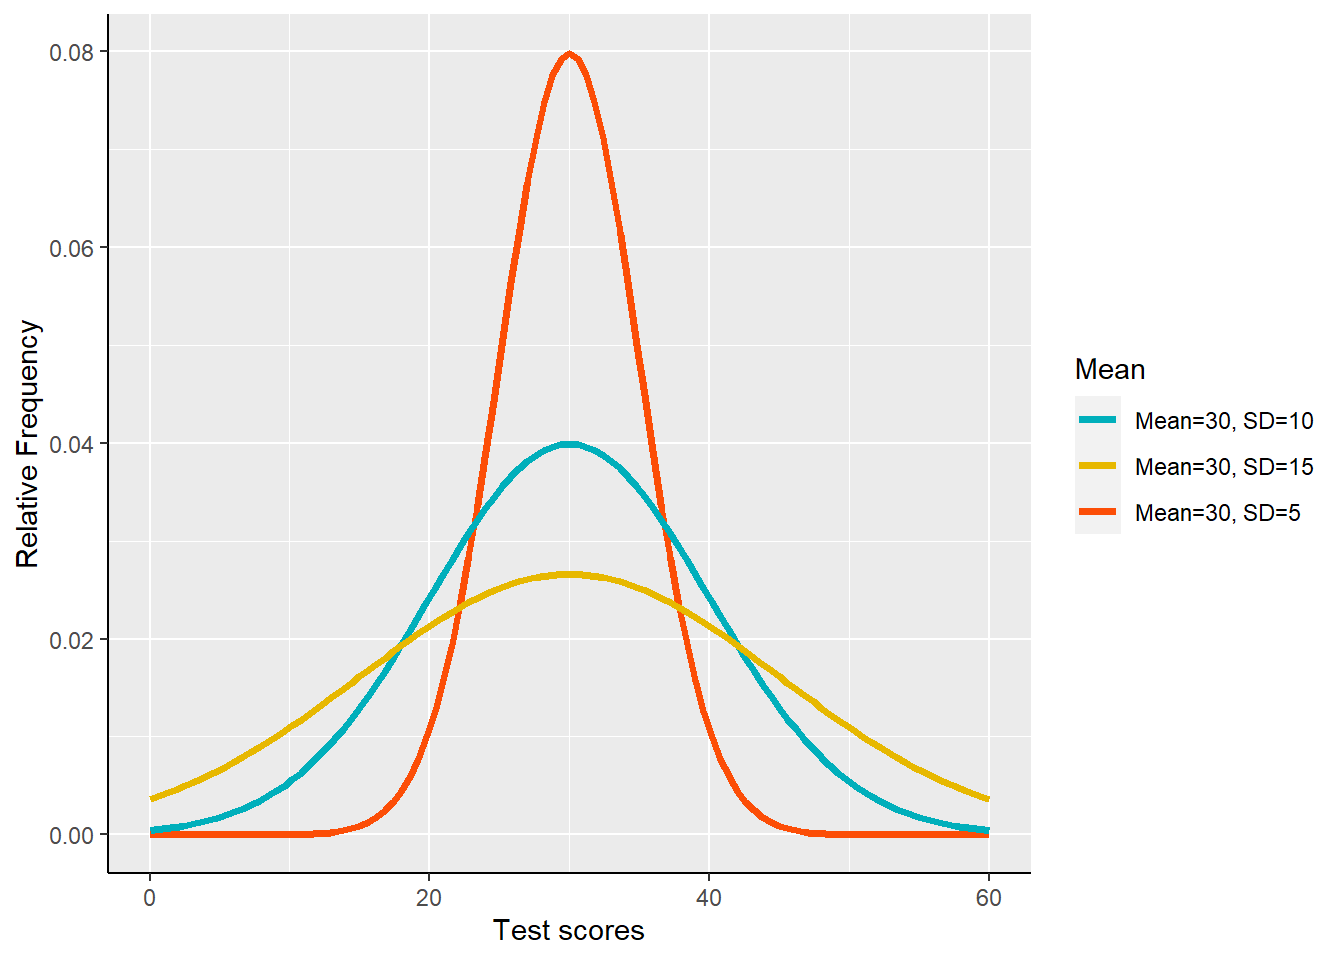
\includegraphics{Bookdown_files/figure-latex/unnamed-chunk-4-1} 

}

\caption{Plot showing several distributions of simulated test score data the same means but differing standard deviations.}\label{fig:unnamed-chunk-4}
\end{figure}

For a mean of 30 and standard deviation of 5: 68\% of the values will lie within the range 25-35.

For a mean of 30 and standard deviation of 10: 68\% of the values will lie within the range 20-40.

For a mean of 30 and standard deviation of 15: 68\% of the values will lie within the range 15-45.

This is particularly clear with a mean of 30 and a standard deviation of 5 as most of the values are tightly packed within the range 25-35.

\hypertarget{example-9}{%
\subsubsection{Example}\label{example-9}}

Calculate the sample estimate of variance and sample estimate of standard deviation for the following list of values:

\[ 2, 4, 4, 5, 6.\]

Start by finding the mean of the values in the dataset:

\[ \textrm{Mean}= \frac{2 + 4 + 4 + 5 + 6}{5}=4.2.\]
Find the difference between each recorded value and the mean.

\begin{longtable}[]{@{}rr@{}}
\caption{\label{tab:table8}}\tabularnewline
\toprule
Value & Difference \\
\midrule
\endfirsthead
\toprule
Value & Difference \\
\midrule
\endhead
2 & 2 - 4.2 = -2.2 \\
4 & 4 - 4.2 = -0.2 \\
4 & 4 - 4.2 = -0.2 \\
5 & 5 - 4.2 = 0.8 \\
6 & 6 - 4.2 = 1.8 \\
\bottomrule
\end{longtable}

Square the differences.

\begin{longtable}[]{@{}rrr@{}}
\caption{\label{tab:table9}}\tabularnewline
\toprule
Value & Difference & Squared Difference \\
\midrule
\endfirsthead
\toprule
Value & Difference & Squared Difference \\
\midrule
\endhead
2 & -2.2 & 4.84 \\
4 & -0.2 & 0.04 \\
4 & -0.2 & 0.04 \\
5 & 0.8 & 0.64 \\
6 & 1.8 & 3.24 \\
\bottomrule
\end{longtable}

Sum the squared differences.

\[\textrm{Sum} = 4.84 + 0.04 + 0.04 + 0.64 + 3.24 = 8.8. \]

Divide the sum by the number of values recorded minus one to get the sample estimate of variance.

\[ \textrm{Variance}_{S} = \frac{8.8}{5-1} = 2.2.\]

To get the sample estimate of the standard deviation take the square root of this value:

\[ \textrm{Standard Deviation}_S = \sqrt{ \textrm{Variance}_{S}} = \sqrt{2.2} = 1.48.\]

\hypertarget{using-excel-1}{%
\subsection{Using Excel}\label{using-excel-1}}

Calculating the variance and standard deviation by hand is a long process and due to the number of steps involved it is prone to error. Excel, SPSS, Python and R all have functions which allow users to calculate these descriptive statives and their use is highly recommended over calculating the statistics by hand.

\textbf{Range}

=MAX(start:end)-MIN(start:end)

\textbf{Standard Deviation}

=STDEV.S(start:end)
=STDEV.P(stard:end)

stdev.s() estimates standard deviation based on a sample. stdev.p() calculates standard deviation based on the entire population given as arguments.

\textbf{Variance}

=VAR.S(start:end)
=VAR.P(start:end)

var.s() estimates variance based on a sample. var.p() calculates variance based on the entire population given as arguments.

\hypertarget{levels-of-measurement-quiz}{%
\chapter{Levels of Measurement Quiz}\label{levels-of-measurement-quiz}}

\begin{center}\rule{0.5\linewidth}{0.5pt}\end{center}

If you would like to try and test your knowledge of the various levels of measurement outlined in this chapter you can take the \href{https://view.genial.ly/62867083cd8fd700184ca06f/presentation-quiz}{Levels of Measurement Quiz} below. This quiz isn't scored or recorded anywhere.

\hypertarget{descriptive-statistics-quiz}{%
\chapter{Descriptive Statistics Quiz}\label{descriptive-statistics-quiz}}

\begin{center}\rule{0.5\linewidth}{0.5pt}\end{center}

If you would like to try and test your knowledge of the various levels of measurement outlined in this chapter you can take the \href{https://view.genial.ly/628a683cb8b7d200114d12a0/presentation-quiz-on-measures}{Measures of Central Tendency and Measures of Dispersion Quiz} below. This quiz isn't scored or recorded anywhere.

\hypertarget{data-visualisation}{%
\chapter{Data Visualisation}\label{data-visualisation}}

\begin{center}\rule{0.5\linewidth}{0.5pt}\end{center}

\hypertarget{data-visualisation-1}{%
\section{Data Visualisation}\label{data-visualisation-1}}

Data visualisation is formally defined as the encoding of data using visual cues such as variations in the size, shape and colour of geometric objects (points, lines, bars). The encoding is generally informed by the relationships within the data.

In the bar chart example below the frequencies of different eye colours have been mapped to the heights of the bars.

\begin{figure}

{\centering 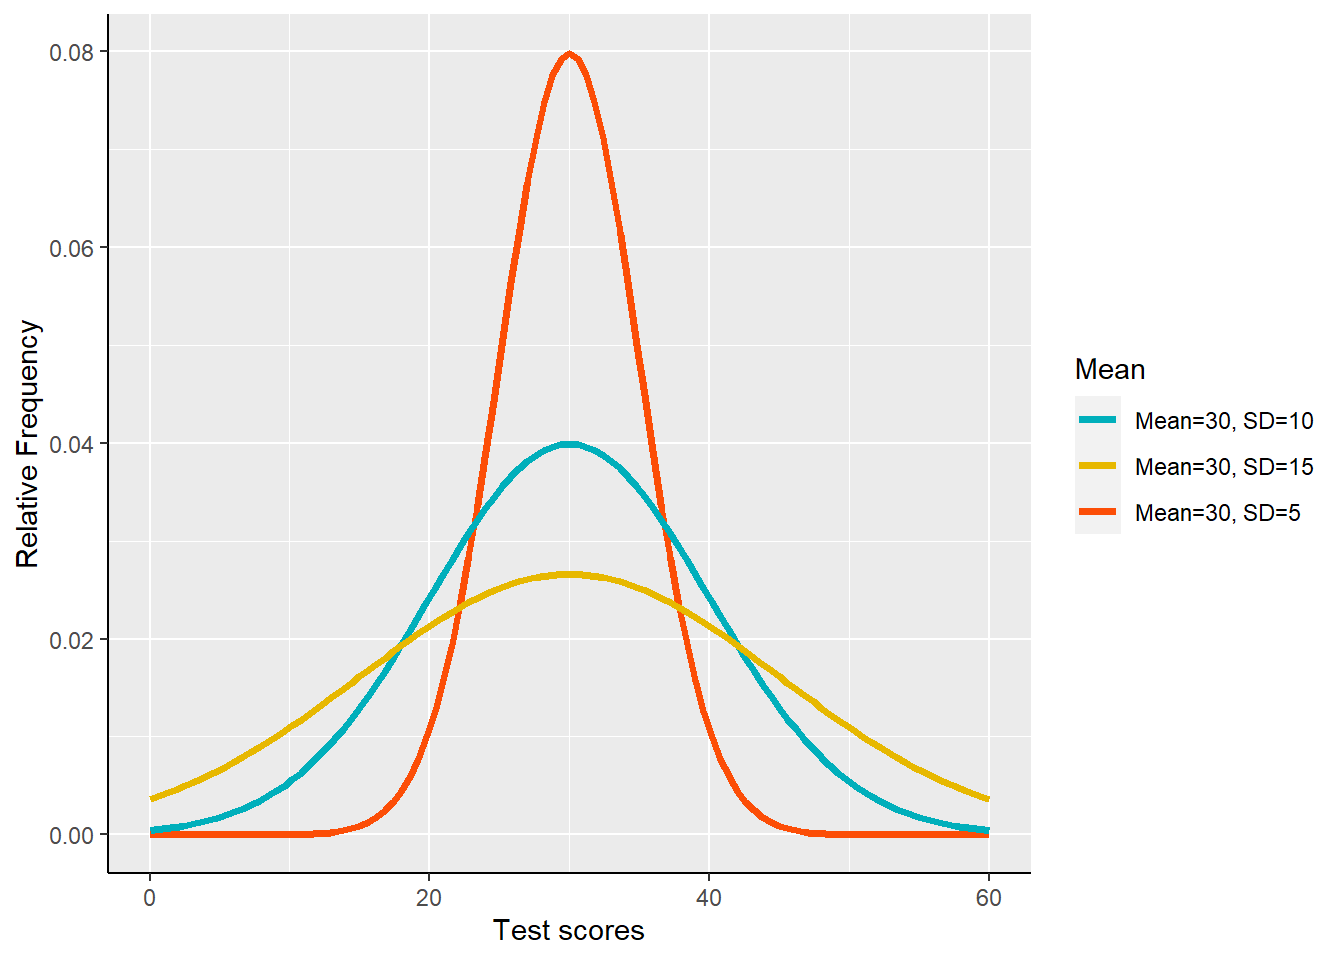
\includegraphics{Bookdown_files/figure-latex/unnamed-chunk-5-1} 

}

\caption{The frequency of each observation has been mapped to the height of the bars in the visual.}\label{fig:unnamed-chunk-5}
\end{figure}

\hypertarget{visual-cues}{%
\section{Visual Cues}\label{visual-cues}}

Whether data is visualised using points, lines, bars or something else entirely is largely determined by the relationships within the data. Some of the visual cues and relationships used to inform data visualisation are shown below.

The illustration above shows some of the visual cues used to encode data. Magnitudes are typically mapped to sizes of objects. Colour is often used to represent quantities or highlight data. Shapes can be used to represent qualitative data.

\hypertarget{relationships-in-data}{%
\section{Relationships in Data}\label{relationships-in-data}}

The \href{https://analysisfunction.civilservice.gov.uk/policy-store/data-visualisation-charts/\#section-9}{Government Statistical Service} has produced guidance on the relationships in data and how they inform chart choices. The guidance can be useful and some of the key points are summarised below.

\hypertarget{frequency-distributions}{%
\subsection{Frequency Distributions}\label{frequency-distributions}}

A histogram or bar chart may be used to show category frequencies. Population by age band for instance could be visualised using a histogram or bar chart in most cases. A boxplot can also be useful in visualising additional statistics such as the mean, median, quartiles, outliers and range.

\begin{figure}

{\centering 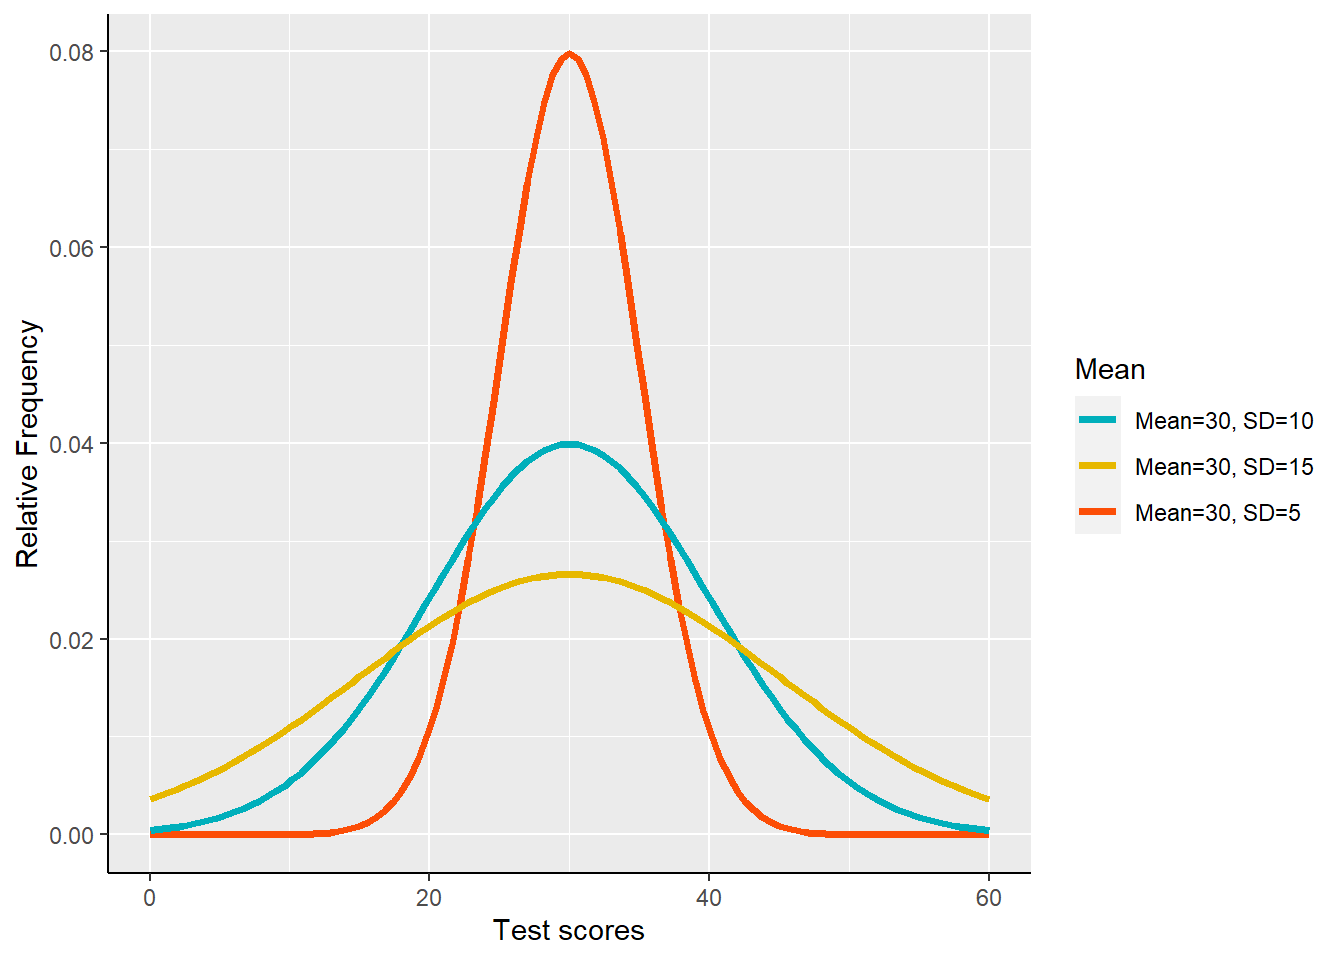
\includegraphics{Bookdown_files/figure-latex/unnamed-chunk-6-1} 

}

\caption{Simulated weight data illustrating the use of a histogram.}\label{fig:unnamed-chunk-6}
\end{figure}

\hypertarget{time-series}{%
\subsection{Time Series}\label{time-series}}

A line chart is often used to demonstrate the trend of a single variable over some time period. Inflation over a ten year time frame for instance can be visualised with a line chart.

\begin{figure}

{\centering 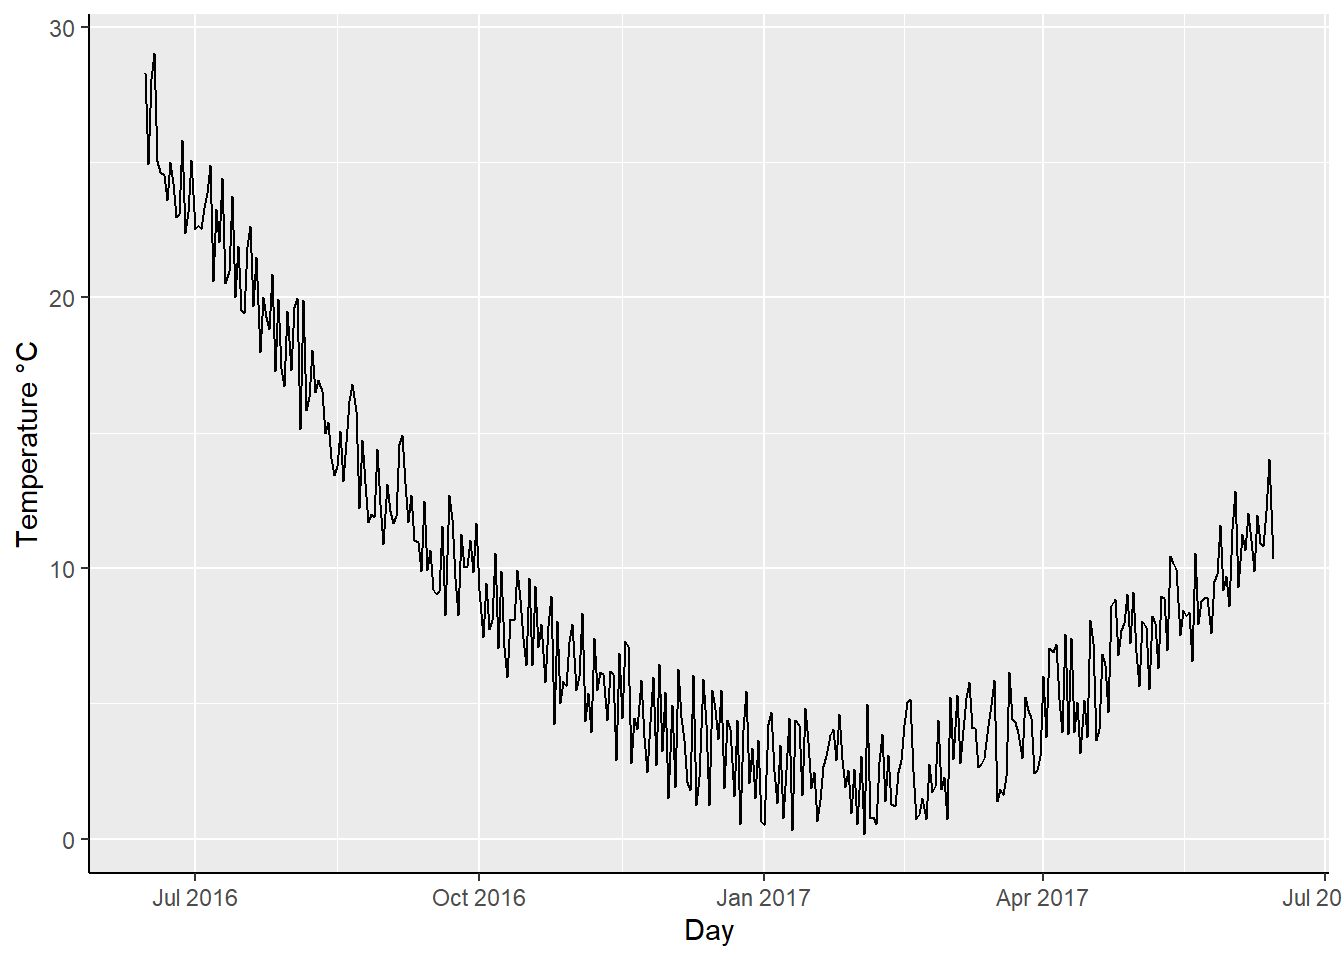
\includegraphics{Bookdown_files/figure-latex/unnamed-chunk-7-1} 

}

\caption{Simulated temperature data.}\label{fig:unnamed-chunk-7}
\end{figure}

\hypertarget{rankings}{%
\subsection{Rankings}\label{rankings}}

Data that is ranked usually consists of categories presented in ascending or descending order. A bar chart may be used to show the comparisons. Sometimes, change in ranking over time is shown through slope charts but usually only when comparing a start date and an end date without consideration for the time period in between.

\hypertarget{deviation}{%
\subsection{Deviation}\label{deviation}}

Deviation from a reference value can be shown through bar charts.

\hypertarget{correlation}{%
\subsection{Correlation}\label{correlation}}

Correlation is usually visualised using scatterplots. Scatterplots are a good way to show comparisons between observations of two variables to determine if there is some correlation.

\begin{figure}

{\centering 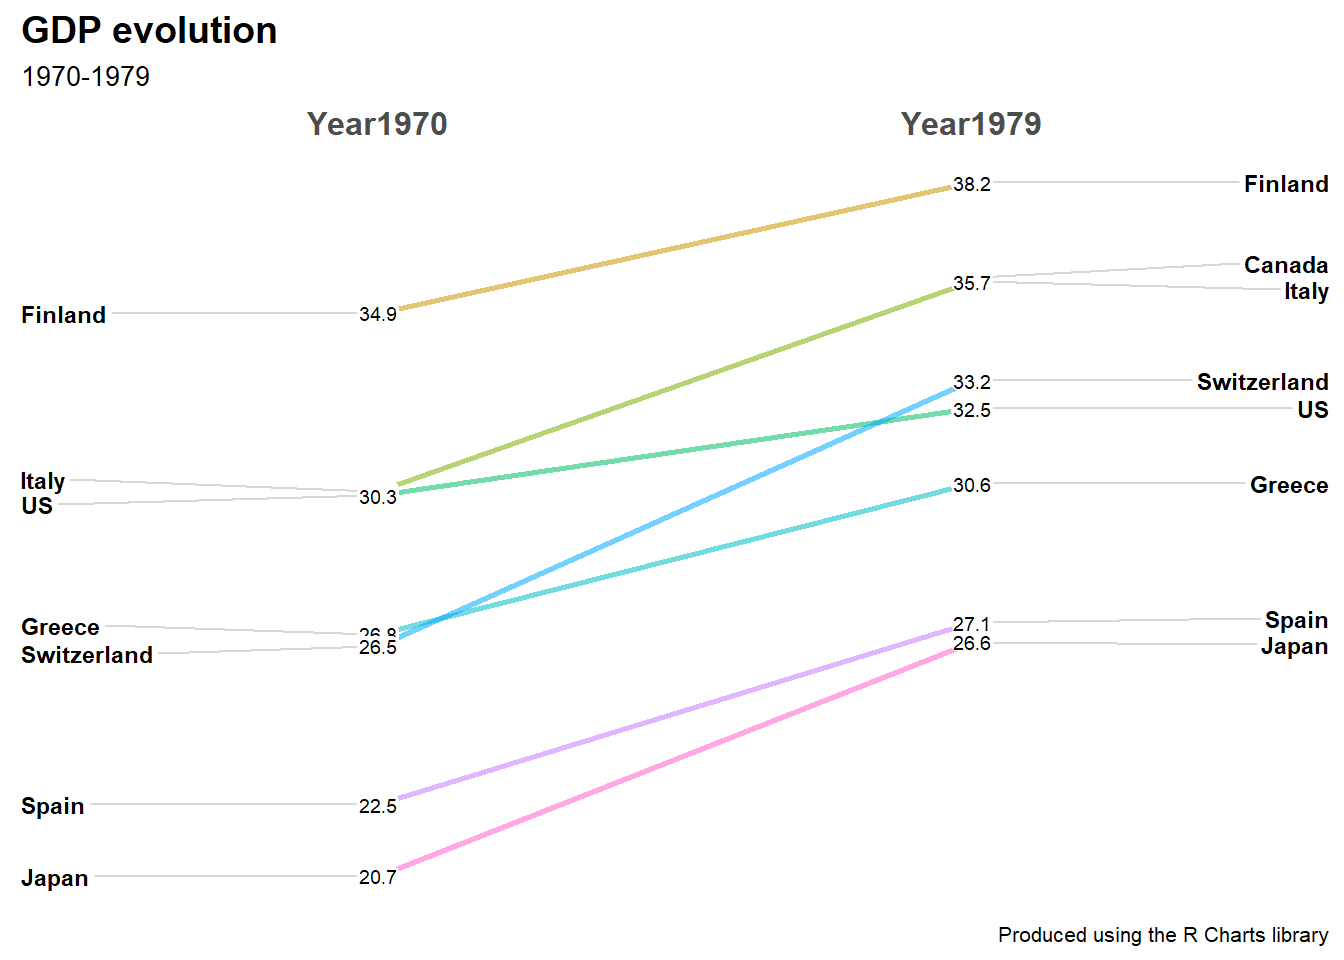
\includegraphics{Bookdown_files/figure-latex/unnamed-chunk-8-1} 

}

\caption{The scatterplot above shows metabolic rate plotted against body weight (kg). This is an example of correlation. This data comes from the Introduction to Statistics with R (ISwR) library for R.}\label{fig:unnamed-chunk-8}
\end{figure}

\hypertarget{magnitude}{%
\subsection{Magnitude}\label{magnitude}}

Comparing differences in the magnitudes of values often relies on bar charts. Comparing the total number of sales by branch for instance.

\hypertarget{spatial}{%
\subsection{Spatial}\label{spatial}}

Cartograms and heat mapping are common ways to show differences between geographical regions.

\hypertarget{why-visualise-data}{%
\section{Why Visualise Data?}\label{why-visualise-data}}

In general, people are better at recognising differences in shapes, colours and sizes than they are at identifying the number of times a value occurs or the differences between values in a large excel spread sheet. For this reason data visualisation can be used to find errors in data quickly. It's much easier to recognise an anomalous value on a bar chart than in an Excel spread sheet. Data visualisation can also be used to see patterns that are difficult to determine by looking at raw data.
Data visualisation can also be used to:

\begin{itemize}
\tightlist
\item
  Answer research questions.
\item
  Discover new research questions.
\item
  Explain complex relationships in data visually.
\item
  Aid in decision making.
\item
  Engage and inform.
\end{itemize}

\hypertarget{data-visualisation-tools}{%
\section{Data Visualisation Tools}\label{data-visualisation-tools}}

New programming languages and software products have made data analysis and visualisation vastly more accessible. In addition, many of these facilitate dynamic or interactable visualisations. There is an ever expanding ecosystem of data visualisation tools (many of which have been used in this document) including:

\begin{itemize}
\tightlist
\item
  \textbf{Excel} and \textbf{SPSS} produce high quality visualisations and while dynamic visuals are not their focus they are often the simplest and most time efficient option for visualising data.
\item
  \textbf{Genially} is an online tool for creating interactive and animated content that is particularly effective for presentations.
\item
  \textbf{Tableau} and Power BI are visual analytics platforms which are well suited to the development of dashboards to visualise complex interconnected data sets.
\item
  \textbf{Flourish} can be used to produce interactive visuals although its functionality is more limited than Power BI or Tableau.
\item
  \textbf{Javascript} facilitates data visualisation through its D3 library. D3 has a steep learning curve as it requires JavaScript skills to use it effectively however it offers a greater degree of customisation and a broader spectrum of visualisation options as a result.
\item
  \textbf{Python} libraries such as Matplotlib, Seaborn and Plotly can also be used to visualise data. The learning curve is steep as it requires programming skills to use Python effectively however Python offers customisation options that are not available in Excel or Power BI.
\item
  \textbf{R} is another useful tool with libraries such as ggplot2 which can be used to visualise data. This is the programming language used to develop this resource and many of the visualisations throughout.
\end{itemize}

\hypertarget{dynamic-visualisations-dashboards}{%
\section{Dynamic Visualisations (Dashboards)}\label{dynamic-visualisations-dashboards}}

There are a number of considerations when developing dynamic data visualisations for a parliamentary audience as not all data visualisations need to be dynamic.
Considering the audience, objectives and what visuals will be most appropriate to communicate data can help in determining whether a dynamic or interactive visualisation is needed.

Dashboard style visualisations are best suited to data reporting where there is a need to repeatedly produce the same visuals or reports either daily, monthly, quarterly or annually.

Power BI is well designed for these types of visualisation requirements as it offers automation options enabling data sets to be refreshed at regular time intervals.
Automation can be as simple as setting a refresh time in the Power BI dashboard and manually updating the excel file it stores in memory or it can be more complex and involve using programming languages to make API calls and perform automated calculations.

Producing dynamic visualisations is often considerably more time expensive than producing static visuals and time constraints should be considered before developing a dashboard visualisation.

\hypertarget{best-practice}{%
\subsection{Best Practice}\label{best-practice}}

GSS have produced \href{https://gss.civilservice.gov.uk/policy-store/top-tips-for-designing-dashboards/}{guidance on designing dashboards} that covers most aspects of dashboard design. The content below summarises some of the key points in this guidance.

\textbf{Consider Audience and User Needs}

Consider the user needs and whether a dashboard is really needed. Often the simplest solution (bar charts drawn in Excel or SPSS) is the best. Consider the visuals used and whether they're the best way to communicate the data. Sometimes tables, text or annotations are better.

\textbf{Guidance}

Providing guidance is important as many users will not be familiar with interactive dashboards. Guidance can be provided in documentation, blog text or it can be provided through tool tips and information pages in the dashboard itself.

\textbf{Streamline Content}

When adding any new data or visuals it is important to ask whether it adds value. Try to group related content and streamlining the content to guide the users through the data.

\textbf{Automate }

Automation can be simple or complex, it can be achieved by setting a refresh date in a Power BI dashboard. It can also involve the use of programming languages to make API calls, web scrape data and perform calculations. Automation typically results in less manual updating and a reduced chance of error and can make the management of the product less resource intensive.

\textbf{Consider Design Principles}

Give your dashboard a header and dedicated areas for visuals. Consider other dashboards you have seen in the past and draw inspiration from web design. Most websites have a navigation bar at the top, lists with filters along the left or right hand side and content in the center of the page. Think about things like symmetry, flow and a consistent style or layout. Use white space where possible and try to avoid cluttered visualisations.

\textbf{Ensure Accessibility}

Ensure your product is accessible by checking the colour contrast ratios of text and including alt text in your visualisations where possible. Ensure the fonts are large enough to read and avoid using multiple fonts.

\hypertarget{comparing-data}{%
\chapter{Comparing Data}\label{comparing-data}}

\begin{center}\rule{0.5\linewidth}{0.5pt}\end{center}

\hypertarget{percentage-change}{%
\section{Percentage Change}\label{percentage-change}}

Percentage change is about comparing old to new values. The formula for calculating a percentage change is given below:

\[ \textrm{Percentage Change} = 100\% \frac{\textrm{New Value} - \textrm{Old Value}}{\textrm{Old Value}}\]
\#\#\# Example

What is the percentage change in the claimant count in these three wards between 2018 and 2019?

\begin{longtable}[]{@{}rrrr@{}}
\caption{\label{tab:table10}}\tabularnewline
\toprule
Ward & 2018 & 2019 & Percentage Change (\%) \\
\midrule
\endfirsthead
\toprule
Ward & 2018 & 2019 & Percentage Change (\%) \\
\midrule
\endhead
Upper Braniel & 50 & 36 & -28 \\
Donaghmore & 50 & 50 & 0 \\
Tobermore & 50 & 58 & 16 \\
\bottomrule
\end{longtable}

Use the formula above to calculate the percentage change for Upper Braniel:

\[ \textrm{Percentage Change} = 100\% \frac{\textrm{New Value} - \textrm{Old Value}}{\textrm{Old Value}}\]

\[ \textrm{Percentage Change} = 100\% \frac{36 - 50}{50} = 100\% \frac{-14}{50} = -28\%\]
A negative percentage change indicates a percentage decrease while a positive percentage change indicates a percentage increase.

\hypertarget{percentage-point-change}{%
\section{Percentage Point Change}\label{percentage-point-change}}

Note that subtracting one percentage from another gives the percentage point change rather than the percentage change.

\hypertarget{example-10}{%
\subsection{Example}\label{example-10}}

What is the percentage point change in the claimant count in these wards between 2018 and 2019?

\begin{longtable}[]{@{}rrrr@{}}
\caption{\label{tab:table11}}\tabularnewline
\toprule
Ward & 2018 & 2019 & Percentage Change (\%) \\
\midrule
\endfirsthead
\toprule
Ward & 2018 & 2019 & Percentage Change (\%) \\
\midrule
\endhead
Upper Braniel & 3.5 & 2.5 & -1 \\
Donaghmore & 3.4 & 3.3 & -0.1 \\
Tobermore & 3.3 & 3.8 & 0.5 \\
\bottomrule
\end{longtable}

\hypertarget{rates}{%
\section{Rates}\label{rates}}

Rates are common in demography, e.g., births per 1,000 persons, deaths by cause per 100,000 persons.

They allow for comparisons between areas with different population sizes.

\hypertarget{example-11}{%
\subsection{Example}\label{example-11}}

In 2012 there were 212 domestic burglaries in Antrim. In the same year, there were 362 Craigavon. At a glance it might appear that burglary is more common in Antrim however the burglary rates per 10,000 persons are very similar (39 and 38 respectively).

  \bibliography{book.bib,packages.bib}

\end{document}
